\section{Research Method}
\label{sec:research-method}

The methodology is organized as a sequential computational framework that links verified sample construction to volatility modelling, option-response formulation, and global sensitivity analysis. The subsections below first describe the research design and data, then present return diagnostics and the GJR-GARCH specification, formulate the Black--Scholes response and transaction-cost loading, explain the Sobol design, and finally document the reproducibility and robustness procedures that support the analysis.

\subsection{Research Design and Data}
\label{subsec:research-design}

This study is a computational mathematical-finance study. Its objective is not to claim improved pricing accuracy against observed option quotations, but to decompose the variation of a model-generated European call-option response. The workflow consists of official Index X constituent verification, adjusted-price processing, return diagnostics, GJR-GARCH volatility estimation, Black--Scholes response evaluation, and Sobol global sensitivity analysis.

Index X is selected because it is an officially evaluated group of relatively liquid and large-capitalization Indonesian stocks. This makes the index a traceable and market-relevant universe for a controlled option-response experiment, while the official evaluation announcements provide an auditable sampling basis. The final sample contains 19 constituents that remained present in every verified Index X evaluation announcement overlapping the February 2022--December 2025 window; they are denoted Stock A through Stock S. Historical adjusted closing prices are obtained from a public financial-data provider. The consistent-constituent rule creates potential survivorship bias because stocks entering or leaving Index X during the window are excluded; this is accepted to obtain a balanced, consistently verified panel.

The masking protocol is retained for a substantive reporting reason. The stock-level quantities in this study are outputs of a deliberately simplified response experiment and should not be read as issuer-quality, risk-rating, or investment-performance comparisons. Associating named issuers with extreme volatility, residual ARCH, or sensitivity ranks would create a realistic risk of interpretation beyond the model's evidential scope. Masking the names therefore limits the claim to the mathematical mechanism being studied and reduces recommendation-like or reputational inference. Reproducibility is not abandoned: a confidential crosswalk from Stock A--Stock S to the public source identifiers, together with the Index X identity and official constituent documents, is maintained for verification by the editor and reviewers.

The February 2022 starting point is the earliest period for which the official Index X files used in the verification procedure could be consistently extracted and cross-checked. This choice prioritizes constituent verification and comparability over a longer but less consistently documented window. Let $S_t$ denote the adjusted closing price at trading day $t$. The daily logarithmic return is
\begin{equation}
  r_t = \ln\left(\frac{S_t}{S_{t-1}}\right).
  \label{eq:log-return}
\end{equation}
\Eqref{eq:log-return} transforms the adjusted price series into the return series used in all subsequent stationarity, ARCH, and volatility analyses.

The complete sequence of data preparation, volatility estimation, response construction, and sensitivity analysis is summarized in Fig.~\ref{fig:research-design-flowchart}.
\begin{figure}[H]
  \centering
  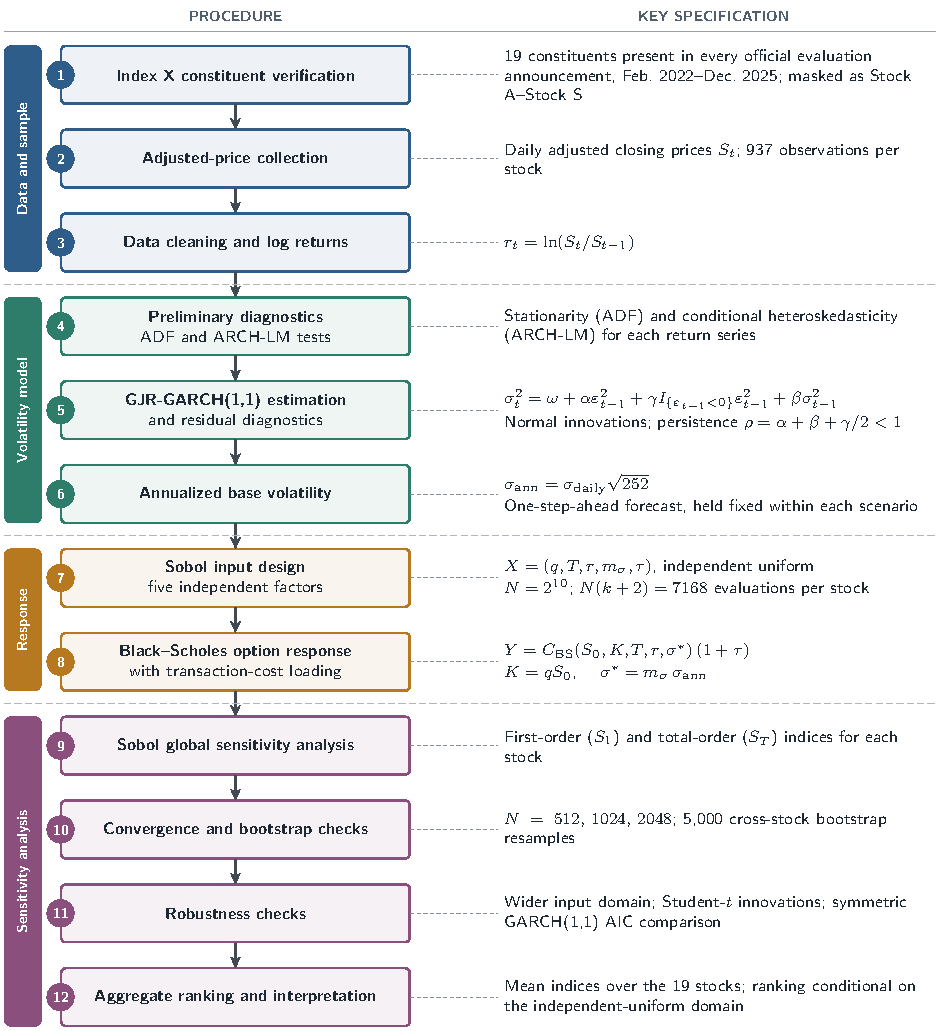
\includegraphics[width=\textwidth,keepaspectratio]{figures/article2_research_design_flowchart.pdf}
  \caption{Black--Scholes--GJR-GARCH--Sobol research design}
  \label{fig:research-design-flowchart}
\end{figure}

\subsection{Preliminary Tests and GJR-GARCH Model}
\label{subsec:gjr-garch}

Descriptive statistics are computed for each return series. The Augmented Dickey--Fuller test evaluates stationarity, and the ARCH-LM test evaluates conditional heteroskedasticity. Stock C is retained even though its preliminary ARCH-LM result is not significant at 5\%, because it satisfies the same official constituent rule as the other stocks; this exception is reported rather than used to alter the common modelling pipeline.

The conditional-mean relation is given in \Eqref{eq:return-equation}, while \Eqref{eq:gjr-garch} defines the asymmetric conditional-variance recursion:
\begin{equation}
  r_t = \mu + \varepsilon_t,\qquad \varepsilon_t=\sigma_t z_t,
  \label{eq:return-equation}
\end{equation}
and
\begin{equation}
  \sigma_t^2 = \omega + \alpha\varepsilon_{t-1}^{2}
  +\gamma I_{\{\varepsilon_{t-1}<0\}}\varepsilon_{t-1}^{2}
  +\beta\sigma_{t-1}^{2}.
  \label{eq:gjr-garch}
\end{equation}
The baseline specification uses a constant conditional mean and normally distributed standardized innovations. GJR-GARCH is chosen as a common flexible specification because it nests the symmetric response when $\gamma=0$, permits leverage asymmetry when the data support it, and allows the same diagnostic pipeline to be applied without selecting a different model after observing each stock's significance result. The choice is evaluated through parameter significance, residual ARCH tests, persistence, a symmetric-GARCH AIC comparison, and a Student-$t$ innovation check. The persistence measure is $\rho=\alpha+\beta+\gamma/2$, with covariance-stationarity requiring $\rho<1$. The one-step-ahead daily volatility forecast is converted to an annualized base volatility by \Eqref{eq:annualized-volatility}:
\begin{equation}
  \sigma_{\mathrm{ann}}=\sigma_{\mathrm{daily}}\sqrt{252}.
  \label{eq:annualized-volatility}
\end{equation}

This annualized value is held fixed as the base volatility inside each contract scenario. The reason for using one common as-of-date volatility signal is to isolate the Sobol contribution of the contract inputs under an identical information set; allowing the volatility forecast itself to evolve with $T$ would make volatility horizon-dependent and mix the maturity effect with variance dynamics. This design is suitable for a controlled sensitivity experiment, but it is a Black--Scholes response with a GJR-GARCH-based volatility input, not a full GJR-GARCH option-pricing model. It is not equivalent to a multi-step forecast or an expected average conditional variance over a maturity of up to one year. A horizon-consistent construction is the appropriate extension when the objective changes from factor isolation to market-consistent valuation across maturities.

Post-estimation ARCH-LM tests are applied to standardized residuals. As robustness checks, the same return series are re-estimated with Student-$t$ innovations, and the normal-innovation GJR-GARCH is compared with a symmetric GARCH(1,1) specification using AIC. The robustness outputs are generated by \texttt{scripts/15\_article2\_reviewer\_robustness.py} and do not replace the baseline results.

\subsection{Black--Scholes Response and Transaction-Cost Loading}
\label{subsec:response-function}

For each Sobol scenario, define the moneyness ratio as $q=K/S_0$ and the effective volatility as $\sigma^*=m_\sigma\sigma_{\mathrm{ann}}$, where $m_\sigma$ is the volatility multiplier. The symbols $q$ and $m_\sigma$ are deliberately distinct: $q$ determines the relative strike through $K=qS_0$, whereas $m_\sigma$ scales only volatility. The European call value is then computed with the effective scenario volatility in \Eqref{eq:black-scholes-call}:
\begin{equation}
  C_{\mathrm{BS}}=S_0N(d_1)-Ke^{-rT}N(d_2),
  \label{eq:black-scholes-call}
\end{equation}
where the standardized terms are defined by \Eqref{eq:d1-d2}:
\begin{equation}
  d_1=\frac{\ln(S_0/K)+(r+\tfrac12(\sigma^*)^2)T}
  {\sigma^*\sqrt{T}},\qquad
  d_2=d_1-\sigma^*\sqrt{T}.
  \label{eq:d1-d2}
\end{equation}

To include a controlled transaction-cost factor without claiming a general frictional pricing model, the simulated Sobol response is defined explicitly in \Eqref{eq:response-function} as
\begin{equation}
  Y=C_{\mathrm{BS}}(S_0,K,T,r,\sigma^*)(1+\tau),
  \label{eq:response-function}
\end{equation}
where $\tau$ is a proportional loading. The loading is retained because the research question requires a transparent, bounded cost perturbation while preserving the closed-form Black--Scholes response and a separately identifiable Sobol input. It is a scenario surcharge, not a structural claim about hedging costs. Transaction costs in option pricing generally affect replication, hedging, or boundary conditions and cannot generally be represented by this multiplication. Accordingly, the small transaction-cost Sobol index is partly induced by the multiplicative form and selected $[0,0.02]$ range and is interpreted only as a property of this experiment, not as a general conclusion that transaction costs are unimportant.

\subsection{Sobol Global Sensitivity Analysis}
\label{subsec:sobol-method}

The uncertain inputs are $X=(X_1,\ldots,X_5)$, consisting of moneyness $q=K/S_0$, maturity $T$, risk-free rate $r$, volatility multiplier $m_\sigma$, and transaction cost $\tau$. Each input is assumed to be independent and uniformly distributed over the corresponding interval. Uniform distributions are used because the experiment specifies plausible bounds but has no defensible empirical density for hypothetical option contracts; equal weighting avoids imposing an unsupported concentration around a preferred scenario and makes the conditional interpretation transparent. The symbols, units, and baseline ranges are reported in Table~\ref{tab:sobol-input-ranges}.
\begin{table}[H]
  \centering
  \caption{Independent-uniform input domain for Sobol analysis}
  \label{tab:sobol-input-ranges}
  \begin{tabular}{lll}
    \toprule
    Input factor & Symbol & Uniform range \\
    \midrule
    Moneyness & $q=K/S_0$ & $[0.90,1.10]$ \\
    Maturity & $T$ & $[1/12,1]$ year \\
    Risk-free rate & $r$ & $[0.04,0.07]$ \\
    Volatility multiplier & $m_\sigma$ & $[0.75,1.25]$ \\
    Transaction cost & $\tau$ & $[0.00,0.02]$ \\
    \bottomrule
  \end{tabular}
\end{table}

The use of a policy-rate interval for $r$ is a scenario choice for a computational experiment. The interval supplies a documented domestic monetary-rate scale and a common range across stocks, which supports controlled comparison. A maturity-matched government yield would be conceptually more direct for market valuation; therefore the policy rate is not presented as an exact tradable discount curve. The factor ranking is conditional on the independent-uniform domain and is not an empirical joint-distribution result.

For each scenario, $K=qS_0$ and $\sigma^*=m_\sigma\sigma_{\mathrm{ann}}$ are used in Equations~\eqref{eq:black-scholes-call}--\eqref{eq:response-function}. With $N=2^{10}=1024$ and five factors, $N(k+2)=7168$ model evaluations are required per stock. First-order and total-order indices are estimated using the Sobol sequence, and stock-level indices are aggregated by arithmetic mean across the 19 constituents.

Numerical convergence is assessed at $N=512$, $1024$, and $2048$. Bootstrap intervals use 5,000 resamples with seed 20260703. These intervals describe cross-stock variability in the deliberately selected 19-stock panel; they are not sampling-error intervals for a single Sobol estimator and are not population-inference intervals. Numerical stability is assessed separately by the convergence comparison.

As an additional domain check, the wider domain is $K/S_0\in[0.85,1.15]$, $T\in[1/12,1.5]$, $r\in[0.03,0.08]$, $m_\sigma\in[0.50,1.50]$, and $\tau\in[0,0.03]$. The Student-$t$ check propagates Student-$t$ GJR-GARCH forecasts through the same baseline Sobol domain. These checks test whether the qualitative ranking is tied to one innovation distribution or one narrow interval choice.

\subsection{Reproducibility}
\label{subsec:computational-procedure}

Computations use Python, \texttt{pandas}, \texttt{statsmodels}, \texttt{arch}, and \texttt{SALib}. The Sobol seed is 42 and the bootstrap seed is 20260703. The revised submission reports the 19 masked labels, observation window, input distributions, parameter ranges, model assumptions, and robustness outputs. The processed data, scripts, and generated tables use the same masked labels. The confidential identity crosswalk and public-source verification record can be supplied to the editor and reviewers; raw market data remain subject to the provider's terms.
